\documentclass[12pt,a4paper,onecolumn]{article}
\usepackage[utf8]{inputenc}
\usepackage[T1]{fontenc}
\usepackage[french]{babel}

\usepackage{multicol}
\usepackage{fullpage}

% ------------------------- Color table ----------------------------------------
\usepackage{multirow}
\usepackage[table]{xcolor}
\definecolor{maroon}{cmyk}{0,0.87,0.68,0.32}
\usepackage{booktabs} % to make prettier tables (toprule, midrule, bottomrule)
% ------------------------------------------------------------------------------

\usepackage{amscd}
\usepackage{amsthm}
\usepackage{physics}
\usepackage{fullpage}
\usepackage{textcomp,gensymb} %pour le °C, et textcomp pour éviter les warning
\usepackage{graphicx} %pour les images
\usepackage{caption}
\usepackage{subcaption}
\usepackage[colorlinks=true,
	breaklinks=true,
	citecolor=blue,
	linkcolor=blue,
	urlcolor=blue]{hyperref} % pour insérer des liens
\usepackage{epstopdf} %converting to PDF
\usepackage[export]{adjustbox} %for large figures

\usepackage{array}
\usepackage{dsfont}% indicatrice : \mathds{1}


% -------------------------- Mathematics ---------------------------------------
\graphicspath{{images/}{../images/}} % For the images path
% ------------------------------------------------------------------------------

% -------------------------- Mathematics ---------------------------------------
\usepackage{mathrsfs, amsmath, amsfonts, amssymb}
\usepackage{bm}
\usepackage{mathtools}
\usepackage[Symbol]{upgreek} % For pi \uppi different from /pi

% For pseudo-code
\usepackage[ruled,vlined,linesnumbered,noresetcount]{algorithm2e}

\newcommand{\R}{\mathbb{R}} % For Real space
\usepackage{tikz}
\usetikzlibrary{bayesnet} %library to draw graphical models1
% ------------------------------------------------------------------------------


% -------------------------- Code format ---------------------------------------
\usepackage[numbered,framed]{matlab-prettifier}
\lstset{
	style              = Matlab-editor,
	basicstyle         = \mlttfamily,
	escapechar         = '',
	mlshowsectionrules = true,
}
% ------------------------------------------------------------------------------

% ------------------------- Blbiographie --------------------------------------
\usepackage[backend=biber, style=ieee]{biblatex}
\addbibresource{biblio.bib}
\usepackage{csquotes}
% ------------------------------------------------------------------------------


\setcounter{tocdepth}{4} %Count paragraph
\setcounter{secnumdepth}{4} %Count paragraph
\usepackage{float}

\usepackage{graphicx} % for graphicspath
% \graphicspath{{../images/}}

\usepackage{array,tabularx}
\newcolumntype{L}[1]{>{\raggedright\let\newline\\\arraybackslash\hspace{0pt}}m{#1}}
\newcolumntype{C}[1]{>{\centering\let\newline\\\arraybackslash\hspace{0pt}}m{#1}}
\newcolumntype{R}[1]{>{\raggedleft\let\newline\\\arraybackslash\hspace{0pt}}m{#1}}


\usepackage{hyperref}

% \setcounter{section}{5} % to start counting section to 6

% Independent sign
\newcommand{\indep}{\ensuremath{\,\bot\!\!\!\bot\,}} %% The symbol for independent

% Alpha / Numbers for sections
\renewcommand{\thesubsubsection}{\arabic{section}.\arabic{subsection}.\alph{subsubsection})}

% Norm
\newcommand{\norm}[1]{\left\lVert#1\right\rVert}


% ------------------------ General informations --------------------------------
\title{PGM Intermediary report \\ Latent Dirichlet Allocation}
\author{Quentin LEROY, Vincent MATTHYS, Bastien PONCHON}
\date{December 2017}
% ------------------------------------------------------------------------------


\begin{document}

\begin{center}

	\rule[11pt]{5cm}{0.5pt}

	\textbf{\Large \textsc{PGM Intermediary Report} \\ Latent Dirichlet Allocation}
	\vspace{0.5cm}

	Quentin LEROY, Vincent MATTHYS, Bastien PONCHON\\
	\{qleroy,vmatthys,bponchon\}@ens-paris-saclay.fr

	\rule{5cm}{0.5pt}

	\vspace{1cm}
\end{center}


The paper we are working on is \textbf{Latent Dirichlet Allocation} \textit{by Bley, Ng and Jordan}.

\section{The model}

In this paper, the authors present a generative probabilistic model of a corpus of text documents or of other kinds of collections of discrete data. This model is parametrized by some hyper-parameters $\xi \in \mathbb{R}$, and by a number $k$ of possible topics and a number $V$ of possible words that can be found in the corpus of $M$ documents.  Each corpus $D$ is then parametrized by $\alpha \in \mathbb{R}_{*+}^{k} $, and $\beta \in [0,1]^{k \times V}$, and the model assumes that each document $\bm{w_d}$ of the corpus has been generated as follows:
\begin{enumerate}
	\item The size of the document is $N \sim$ Poisson($\xi$)
	\item The topic mixture parameter $\theta \in [0,1]^{k}, \sum_{i = 1}^{k}\theta_i = 1$ is drawn from Dir($\alpha$)
	\item For each $n \in [1, N]$:
	      \begin{enumerate}
		      \item The topic $z_n \in [0,1]^k$ of the $n^{th}$ word is drawn from Multinomial($\theta$)
		      \item The word $w_n$ is drawn from $p(w_n|z_n, \beta)$ where $p(w_n^j=1|z_n^i=1, \beta) = p(w_k^j=1|z_k^i=1, \beta) = \beta_{ij} \quad \forall k \in [1, N]$
	      \end{enumerate}

\end{enumerate}
The probabilistic graphical model of the representation is shown in Figure~\ref{fig1}. The authors then discuss the assumptions on which this model is built (especially the assumption of exchangeability), compare it with other latent variables models (such as mixture of unigrams), and provide a graphical interpretation.

\begin{figure}[H]
	\centerline{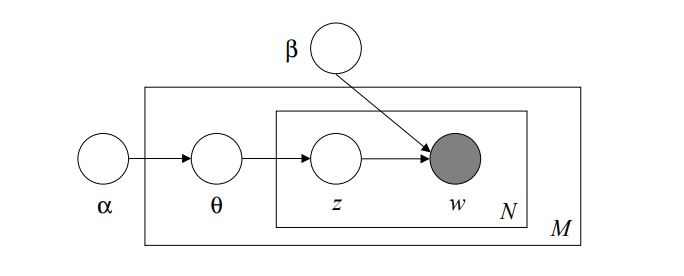
\includegraphics[height = 0.20\textheight]{Figure0.JPG}}
	\caption{Probabilistic graphical model representation of the Latent Dirichlet Allocation model}\label{fig1}
\end{figure}


\section{Inference}

Once we learned the parameters $\alpha$ and $\beta$ of the document corpus, we can use the generative model to estimate the distributions of the hidden variables given a new document: $p(\theta, \bm{z}|\bm{w}, \alpha, \beta)$. However this distribution is intractable, the authors hence have to resort to variational inference to solve it. The idea behind variational inference is to find a lower bound of the log likelihood thanks to a more tractable distribution, shown in figure~\ref{fig2}. The authors show that maximizing this lower bound with regard to the variational parameters $\gamma$ and $\phi$ is equivalent to minimizing the Kullback-Leibler divergence between this approximate distribution and the actual distribution of the LDA. We then have a convex optimization problem in the parameters $\gamma$ and $\phi$, leading to an iterative algorithm to compute their approximated value.

\begin{figure}
	\centerline{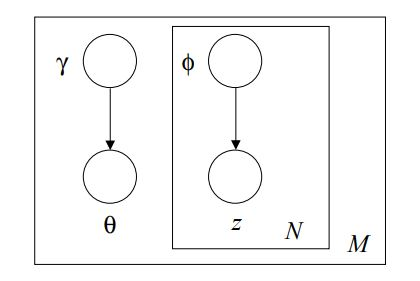
\includegraphics[height = 0.25\textheight]{Figure0_1.JPG}}
	\caption{Graphical model representation of the variational distribution used to approximate the posterior in LDA}\label{fig2}
\end{figure}


\section{Parameters estimation}

Before being able to do inference on new documents, we have to train the model on our corpus of documents, by finding the parameters $\alpha$ and $\beta$ that maximize the marginal log likelihood of the data $\sum_{d=1}^M log(p(\bm{w}_d|\alpha, \beta)$. But as stated above we have a lower bound on this likelihood, depending on $\alpha$ and $\beta$ and on (approximate) variational distributions of parameters $\gamma_d$ and $\phi_d$ (for each document $\bm{w}_d$). We can therefore use a variational EM algorithm to estimate $\alpha$ and $\beta$.
\begin{enumerate}
	\item In the E-step we maximize our lower bound with regard to $\gamma_d$ and $\phi_d$ for each $d\in [1, D]$ as presented in the \textit{Inference} section.
	\item In the M-step, we maximize the resulting lower bound with respect to $\alpha$ and $\beta$, for which we have a closed form depending on the $\gamma_d$ and $\phi_d$.
\end{enumerate}

\section{Details of computations}

\begin{equation}
	\begin{split}
		\ell(\bm{w}, \bm{\alpha}, \bm{\beta}) &= \log p(\bm{w} \mid \bm{\alpha}, \bm{\beta})\\
		&= \log \int_{\bm{\theta}} \sum_{\bm{z}} p(\bm{\theta},\bm{z}, \bm{w} \mid \bm{\alpha}, \bm{\beta}) d\bm{\theta}\\
		&= \log \int_{\bm{\theta}} \sum_{\bm{z}} b(\bm{\theta}, \bm{z}) \frac{p(\bm{\theta},\bm{z}, \bm{w} \mid \bm{\alpha}, \bm{\beta})}{b(\bm{\theta}, \bm{z})} d\bm{\theta}\\
		&\ge \int_{\bm{\theta}} \sum_{\bm{z}} b(\bm{\theta}, \bm{z}) \log \left(\frac{p(\bm{\theta},\bm{z}, \bm{w} \mid \bm{\alpha}, \bm{\beta})}{b(\bm{\theta}, \bm{z})} \right)d\bm{\theta} \quad \text{thanks to Jensen's inequality}\\
		&= \mathbb{E}_{b}\left[\ell_c(\bm{\theta},\bm{z}, \bm{w}, \bm{\alpha}, \bm{\beta})\right] - H(b(\bm{\theta}, \bm{z}))\\
		&= \mathbb{E}_{b}\left[\log p(\bm{\theta},\bm{z}, \bm{w} \mid \bm{\alpha}, \bm{\beta})\right] - \mathbb{E}_{b}\left[\log b(\bm{\theta}, \bm{z})\right]\\
		&= \mathcal{L}(b, \bm{\theta},\bm{z}, \bm{w}, \bm{\alpha}, \bm{\beta})
	\end{split}
\end{equation}

\begin{align}
	b^{(t+1)}                         & = \operatorname{arg}\max_{b} \mathcal{L}(b, \bm{\theta},\bm{z}, \bm{w}, \bm{\alpha}^{(t)}, \bm{\beta}^{(t)}) = p(\bm{\theta}, \bm{z} \mid \bm{w}, \bm{\alpha}, \bm{\beta})                                    \tag{E-step}                                                     \\
	(\bm{\alpha}, \bm{\beta})^{(t+1)} & = \operatorname{arg}\max_{(\bm{\alpha}, \bm{\beta})} \mathcal{L}(b^{(t+1)}, \bm{\theta},\bm{z}, \bm{w}, \bm{\alpha}, \bm{\beta}) = \operatorname{arg}\max_{(\bm{\alpha}, \bm{\beta})} \mathbb{E}_{b}(\ell_c(\bm{\theta},\bm{z}, \bm{w}, \bm{\alpha}, \bm{\beta})) \tag{M-step} \\
\end{align}

Which is equivalent to the following system:

\begin{align}
	b^{(t+1)}                         & = \operatorname{arg}\min_{b} \mathcal{D}(b(\bm{\theta}, \bm{z})\mid\mid p(\bm{\theta},\bm{z}\mid \bm{w}, \bm{\alpha}^{(t)}, \bm{\beta}^{(t)}))          \tag{E-step}                   \\
	(\bm{\alpha}, \bm{\beta})^{(t+1)} & = \operatorname{arg}\min_{(\bm{\alpha}, \bm{\beta})} \mathcal{D}(b^{(t)}(\bm{\theta}, \bm{z})\mid\mid p(\bm{\theta},\bm{z}\mid \bm{w}, \bm{\alpha}, \bm{\beta}))          \tag{M-step} \\
\end{align}

Nevertheless the exact inference is not possible due to the untractable posterior distribution \(p(\bm{\theta},\bm{z}\mid \bm{w}, \bm{\alpha}^{(t)}, \bm{\beta}^{(t)})\). A relaxation of the problem is proposed by introduction of the varational distribution \(q(\bm{\theta}, \bm{z} \mid \bm{\gamma}, \bm{\phi})\):

\begin{align}
	(\bm{\gamma}, \bm{\phi})^{(t+1)}
	                                  & = \operatorname{arg}\max_{(\bm{\gamma}, \bm{\phi})} \mathcal{L}(\bm{\gamma}, \bm{\phi}, \bm{\theta},\bm{z}, \bm{w}, \bm{\alpha}, \bm{\beta})                                                                                \notag     \\
	                                  & = \operatorname{arg}\max_{(\bm{\gamma}, \bm{\phi})} \mathbb{E}_{q}\left[\log p(\bm{\theta},\bm{z}, \bm{w} \mid \bm{\alpha}, \bm{\beta})\right] - \mathbb{E}_{q}\left[\log q(\bm{\theta}, \bm{z})\right]                   \tag{E-step} \\
	(\bm{\alpha}, \bm{\beta})^{(t+1)} & = \operatorname{arg}\min_{(\bm{\alpha}, \bm{\beta})} \mathcal{D}(b^{(t)}(\bm{\theta}, \bm{z})\mid\mid p(\bm{\theta},\bm{z}\mid \bm{w}, \bm{\alpha}, \bm{\beta}))          \tag{M-step}                                                 \\
\end{align}

which leads to the following updates:



\end{document}
